\documentclass{jot}

\usepackage[english]{babel}
\usepackage{microtype} % optional, for aesthetics
\usepackage{tabularx} % nice to have
\usepackage{booktabs} % necessary for style
\usepackage{mathtools}
% \usepackage{graphicx}
% \graphicspath{{./figures/}}
% \usepackage{listings}
% \lstset{...}

% \newcommand\code[1]{\texttt{#1}}
% \let\file\code

\graphicspath{{images/}}


%%% Article metadata
\title{Main project: Song Recommendation System}
\runningtitle{Main project: Song Recommendation System}

\author[affiliation=UiT, nowrap]
    {Madhu Koirala}
    {is a master student in Computer Science at the University of Troms\o. You can contact him at \email{mko075@uit.no}.}

\author[affiliation=UiT, nowrap]
    {\'{A}lvaro Mart\'{i}nez Fern\'{a}ndez}
    { is a master student in Computer Science at the University of Troms\o. You can contact him at \email{afe026@uit.no}.}

\affiliation{UiT}{University of Troms\o, Norway\\
\url{https://uit.no/startsida}}

\runningauthor{Madhu Koirala and \'{A}lvaro Mart\'{i}nez}

\jotdetails{
    year=2020,
}


\begin{document}

\begin{abstract}
Looking for specific information on the internet can be a tedious process nowadays because of the large amount of data that need to be navigated. Looking for media content such as songs or movies can be even harder, since it’s difficult to know if it is the right content. Recommendation systems can help users in the decision process by filtering the content based on the content that the user likes and consumes most. In this project,a song recommendation system using collaborative filtering approach has been implemented. The model consists of several users and each user has a list of songs that the user usually listens to. By using collaborative filtering, song recommendations are done by recommending songs from users with similar taste using Co-occurrence matrix. Also, a simple approach which uses popularity of songs (number of users and listen counts) has been implemented. Both methods show a list of recommended songs for a user and a comparison between them with the help of precision recall curve proves a better performance of similarity-based approach.
\end{abstract}

\keywords{Recommendation System, Recommendation Methods, Music Recommendation, Collaborative Filtering, Co-occurrence Matrix}

\tableofcontents

\section{Introduction}
Recommender systems are essentially a subset of information filtering systems. There are some tools like search engines that help the user filter the content, some examples are Google\footnote{https://google.com} or Yahoo\footnote{https://www.yahoo.com}. Modern systems include recommendation algorithms that automatically filter the content for the user, based on the information that the user has consumed. This is  common in multimedia platforms like Netflix\footnote{https://www.netflix.com} or Spotify\footnote{https://www.spotify.com}. Lists of recommended media are shown to the user with content that may be appealing, based on the user’s interests. This is helpful, for instance, songs of interest are already shown in the suggested list by a recommendation engine . Also finding a film to watch on Netflix can be a cumbersome process, which is automatically filtered by the recommendation systems.

There are different ways to build a recommendation system. Some approaches are by using information based on the user’s preferences, item features, factors such as time, season, etc. In the literature, mostly  three methods are found to implement a recommendation algorithm.

\subsection{Content Based Method}
This method depends on the attributes of objects or items and user profile to make recommendations to its users. An item or object is a product that users interact with. For instance, in a movie recommendation system, the name of the movie is an item or object and the name of actors, the year it was produced and the genre of the movie such as romance, action, comedy, etc constitute the attributes. Refer to the below table to understand how exactly this method works. Table \ref{tab:content-based} presents the name of the movie, user ratings and the properties or attributes of the movie.

\begin{table}[h!]
\begin{tabular}{lllll}
Movie                & User 1 & User 2 & Attribute 1(romance) & Attribute 2(Action) \\
Love for Seven Lives & 4      & 5      & 0.9                   & 0.1                  \\
Against Injustice    & 5      &        & 0.1                   & 0.8                  \\
You n Me             & 4      &        & 0.7                   & 0.2                  \\
Earn Kr 1 Spend 10   &        & 1      & 0.1                   & 0.4                  \\
\end{tabular}
\caption{Content Based Filtering.}
\label{tab:content-based}
\end{table}

To find  if User 2 likes the movie You n Me, consider her profile and the attributes of the movie. She likes Love for Seven Lives, which has high romance and almost no action. Based on this, she has a certain profile. When this profile and the attributes of You n Me are matched, it’s highly likely that she will love this movie. So, this movie can be recommended to her.

Content-based recommender system has the advantage that it does not require information about other users. It only needs to know what the current user is interested in. Also, it can recommend niche products as it analyses the interests of a user only as niche items are the goods specific for a particular customer base. However, there are some disadvantages too. The entire domain of sufficient knowledge of the items, such as genre, texts to explain the item, and other information that can describe the item’s several properties need to be created. Another demerit is it only makes recommendations around the interest of a user based on their profile. If the user also likes some other types of items, it does not know because the user has only a certain type of profile. For example, if a product is  popular among some users, then it may be good to recommend it to the rest of the users also. But this system cannot do so unless the profile matches the attributes of the popular product.

\subsection{Collaborative Filtering}
This technique is entirely based on users' interaction with the items. Based on the ratings they have provided, it calculates similarity between the users. If a similarity is found, for example between A and B users, then, the system recommends the items liked by A to B and vice versa.
Let’s try to make it clear with the help  of an example of a music recommendation system. There are many ways to calculate similarity. Below in Table \ref{tab:collaborative-filtering} presents music user interaction for four users and finds sameness using co-occurrence matrix. In this table, 1 denotes that there has been an interaction and 0 denotes no interaction has happened.

\begin{table}[h!]
\centering
\begin{tabular}{lllll}
Users & Music A & Music B & Music C & Music D \\
M     & 1       & 1       &         &         \\
N     & 1       &         & 1       & 1       \\
O     & 1       & 1       & 1       &         \\
P     & 1       & 1       &         &         \\
\end{tabular}
\caption{Interaction Matrix.}
\label{tab:collaborative-filtering}
\end{table}

\begin{table}[h!]
\centering
\begin{tabular}{lllll}
Users & Music A & Music B & Music C & Music D \\
M     & 0       & 3       & 2       & 1       \\
N     & 3       & 0       & 1       & 0       \\
O     & 2       & 1       & 0       & 1       \\
P     & 1       & 0       & 1       & 0       \\
\end{tabular}
\caption{Co-occurrence Matrix.}
\label{tab:collaborative-filtering2}
\end{table}

Co-occurrence matrix is mostly used for determining item similarity. To calculate this matrix, simply count the co-occurrence or simultaneous occurrence of the two items. For instance, for A and B, both of them are liked by users M, O and P and hence the value 3. Similarly other values are calculated. Now, for recommendation, for movie A, it is determined by the values along its column. So, music similar to A are B,C and D in descending order of similarity (See Table \ref{tab:collaborative-filtering2}).

A more simplistic method to find similarity measures is Jaccard algorithm. Let’s consider two users A and B. They have bought a set of products as shown below.

\[A = \{2,6,8,3\}\]
\[B = \{3,8,6,9,10\}\]
\[Products in common = \{6,8,3\}\]
\[Union of Products = \{2,6,8,3,9,10\}\]
\[Jaccard\;Similarity = \frac{Intersection\;of\;the\;two\;sets}{Union\;of\;two\;sets}\]

One good aspect of collaborative methods is it does not require any domain knowledge as it can recommend an item based on the similarity of users according to their feedback. The other advantage is it may be able to recommend all types of items unlike content-based which always advise similar items. For instance, users A and B and C love folk music. And B and C also like pop music. Looking at the similarity between these users, it might be good to recommend pop music to user A. On the other hand, this system can suffer from ‘cold start’ problem. If a number of interactions between various users and items are available, then only it can recommend an item. But for new items or new users, it does not have any information about users’ likings to give suggestions. Also, it suffers from the problem of sparsity. In a real-world situation where there are millions of items and users, no matter how much interaction has been made but still there can be items and users with a few interactions. This can lead to poor recommendations. The other disadvantage it can have is scalability. It will require huge computation in a practical scenario where there is a huge dataset of users and items and can easily lead to the problem of scaling.

\subsection{Hybrid Method}
This method combines both techniques content-based and collaborative filtering that the individual drawbacks are cancelled out. The following example should explain how a hybrid approach can be better in some particular scenarios. Below, Table  \ref{tab:hybrid} shows item-interaction matrix.

\begin{table}[h!]
\centering
\begin{tabular}{lllll}
 & Love for SL(L) & Against Injust. (A) & You n Me & Earn Kr 1 S 10 (E) \\
User 1     & 1       & 1       & 1         & 0      \\
User 2     & 1       & 0       & 0         & 1      \\
\end{tabular}
\caption{User-Item Interaction Matrix.}
\label{tab:hybrid}
\end{table}

Now the table below, Table \ref{tab:hybrid2}, depicts the co-occurrence matrix.

\begin{table}[h!]
\centering
\begin{tabular}{lllll}
 & L & A & Y & E \\
L     & 1       & 1       & 1         & 0      \\
A     & 1       & 0       & 0         & 1      \\
Y     & 1       & 1       & 0         & 0      \\
E     & 1       & 0       & 0         & 0      \\
\end{tabular}
\caption{Co-occurrence Matrix.}
\label{tab:hybrid2}
\end{table}

If two movies similar to each movie is to be recommended then there are not enough movies for movie E. Based on Table \ref{tab:hybrid2}, movie L is similar to E but one more movie is needed. So, in such cases content-based filtering comes into play. The attributes of E show that it has more action and less romance. Movie having such attributes is Against Injustice. So, this can be the second recommendation. This is how a hybrid approach solves problems faced when only one type of system is implemented.

\section{Background and Related Work (state of the art)}
A music recommendation system is a specialized information retrieval system for multimedia content\cite{chung_kim_2018}. A recommendation system\cite{isinkaye_folajimi_ojokoh_2015} is defined as a system that searches through a large volume of information in order to filter the information based on the personalized preferences of the user. It is also seen as a decision making strategy for users under complex information environments. Originally recommender systems were defined as a way to assist the social process of using recommendations of others in order to make choices when there is not sufficient personal knowledge of the different alternatives\cite{resnick_varian_1997}.

Besides the methods discussed above for recommender systems,  machine learning and deep learning techniques have been used to enhance recommendation algorithms. In a study about recommendation systems\cite{singhal_sinha_pant_2017}, an analysis of the literature shows that machine learning and deep learning has been used especially for collaborative filtering algorithms.

There can be many ways to extract properties or features from the objects of recommendation. This creates a better recommender system like in this study\cite{park_yoo_cho_2006}, where they build a music recommendation system based on the context or environment of the listener such as day, time, temperature, if it is rainy, cloudy or sunny, etc. In another study\cite{ayata_yaslan_kamasak_2018} they even measure the mood of the user by using a galvanic skin response and photoplethysmography.

When analyzing related work about recommendation systems, many studies can be found that use the different methods mentioned before. Content-based systems are mostly used when metadata can be used. For instance in this study\cite{cano_koppenberger_wack_2005} they build a music recommendation system that extracts descriptions related to instrumentation, rhythm and harmony from music audio signals. However in this project the number of times a song is heard by users has been used as a collaborative filtering approach has been used. In some recommendation systems\cite{choi_yoo_kim_suh_2012}\cite{debnath_ganguly_mitra_2008}, both collaborative and content based approaches are used, resulting in a hybrid approach. In this way the advantages from each method are utilized  in order to enhance the accuracy of the recommendation system.

\section{Problem to be solved and Aims}
The goal of this project is to design a music recommendation system. There are many methods of implementing a recommender system. A collaborative filtering algorithm is used as it is the most used approach in the real world.
The problems which were anticipated to be faced to accomplish the goals are as below: These problems  will be further discussed in the discussion part.
\begin{enumerate}
  \item How to implement collaborative filtering approach in a music recommender system?
  \item Which particular algorithm will give the optimum performance in this case?
  \item What kind of dataset is required for training and validation of the model and how to  find the right one?
  \item Which machine learning algorithm is needed to use for the best results?
  \item How is the model trained and validated?
\end{enumerate}

\section{Contribution}
A recommendation system for songs can be practical in many applications and services nowadays. With the Internet, people can easily have access to endless multimedia content like music. Also the potential that there is at the moment to find new music and get good recommendations is enormous thanks to machine learning and recommendation systems. An  example of how to implement a song recommendation system using a collaborative filtering algorithm has been presented.

It has been  implemented using Python and some packages like sklearn and pandas used for machine learning. Also a small graphic user interface has been built that shows potential recommendation songs for a user.

As for the evaluation, a comparison between the collaborative filtering solution with a more primitive one, a popularity based algorithm has been made.

\subsection{Architecture and design}
The song recommendation system is built using a machine learning technique\cite{medium}. The dataset used in the system contains information about users, songs that the users have listened to and how many times they have listened to a particular songs. This dataset comes from the Million Song Dataset\cite{millionsongs} and in particular  two files from this dataset have been used. The first dataset\footnote{https:\/\/static.turi.com\/datasets\/millionsong\/song\_data.csv} is the metadata file which contains song ID and related information about the songs. The second one\footnote{https:\/\/static.turi.com\/datasets\/millionsong\/10000.txt} is the rating dataset containing the user ID, song ID and the number of times the songs have been heard by the users. In the system the dataset is trained and it makes 2 types of recommendations, one that is popularity based and a second one that is personalized for each user. Figure \ref{fig:architecture} shows an overview of the architecture of the system.\\

\begin{figure}[h!]
    \centering%
    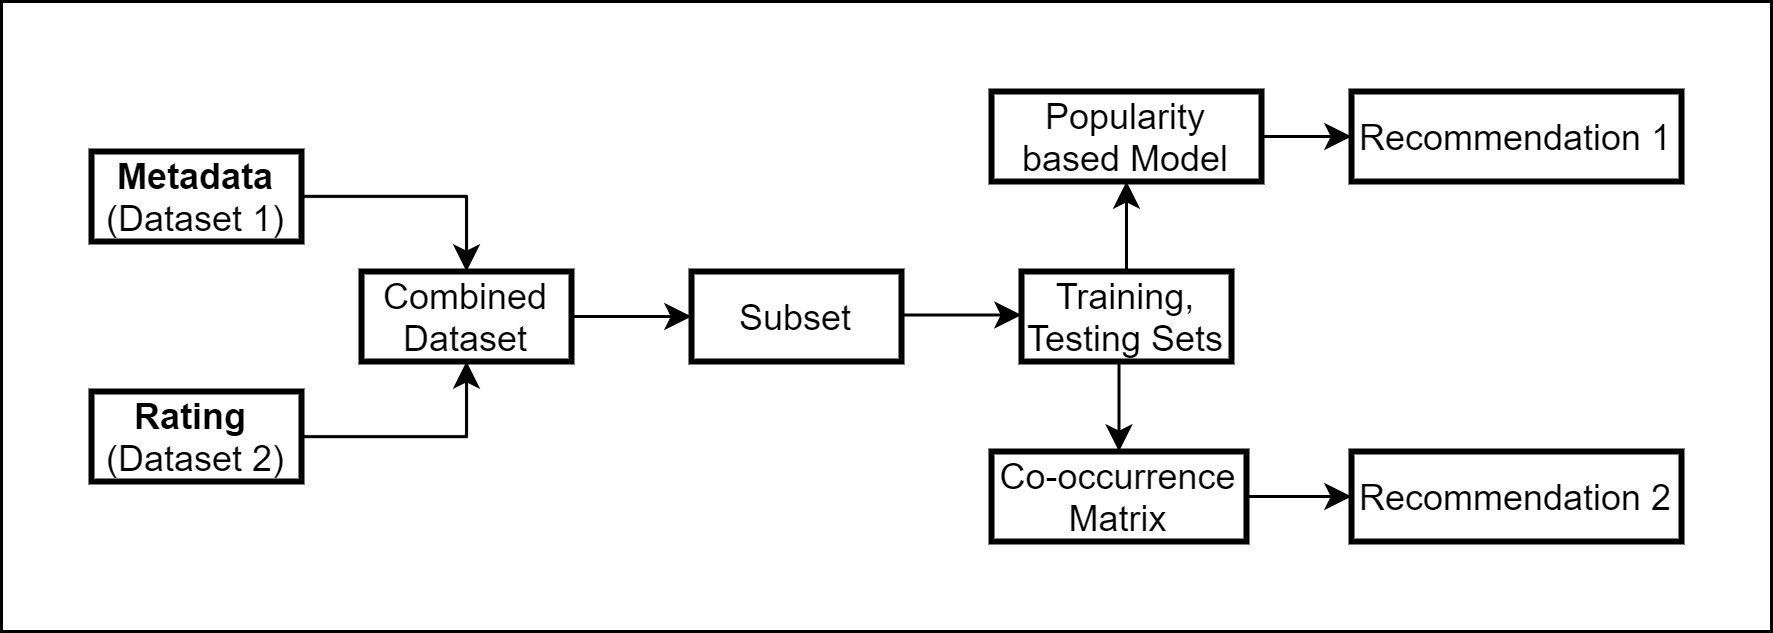
\includegraphics[width=\textwidth]{architecture}
    \caption{Architecture of the system.}
    \label{fig:architecture}
\end{figure}%

The initial step is to combine the two datasets and then remove duplicates that this merging causes and ending up with a new dataset that contains the following fields: User ID, Song ID, Listen Count, Song Title, Release, Artist Name and Release Year. Then a subset of 15000 entries from the dataset is taken since the original dataset is too large and for the purpose of this project it is enough with a smaller dataset. The subset is further split into two sets: training and testing sets, the former comprising 80\% of the dataset. The training set is fed into two models-popularity-based and co-occurrence matrix -based which makes recommendations separately. The training is done only once so it is 1 epoch of training.

For recommendation, two strategies have been adopted. The first one is based on the popularity of songs which is directly related to the number of songs that have been listened to. And the second uses co-occurrence matrix which is a measure that calculates by what factor the items are related to each other.

The popularity based model generates the same results irrespective of the user because it simply lists out the most popular songs. On the other hand, the co-occurrence matrix generates a personalized list of recommended songs for a specific user.

As for the design of the system, Python has been used to develop the song recommendation system. For the machine learning logic, pandas and sklearn Python packages have been used. pandas is a data analysis and manipulation tool that helped us shape the dataset. sklearn was used to train the dataset using the function train\_test\_split, which split arrays or matrices into random train and test subsets.

A small graphic user interface using the tkinter Python package has also been built, which is used for graphic interfaces. The GUI can show the song recommendation for a particular user, using the co-occurrence matrix approach. See Figure \ref{fig:design} for an example of the GUI.

\begin{figure}[h!]
    \centering%
    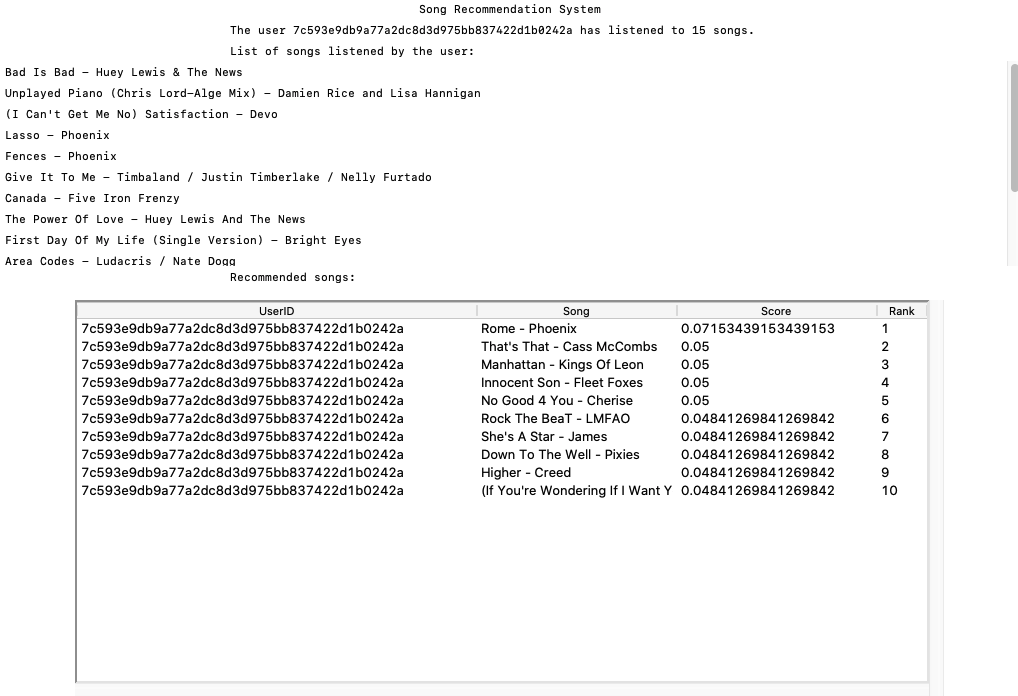
\includegraphics[width=\textwidth]{design}
    \caption{GUI for song recommendation for a particular user using the co-occurrence matrix approach.}
    \label{fig:design}
\end{figure}%

\subsection{Results and evaluation}
The program is able to produce recommendations for both popularity-based and similarity based approaches. Both of them provide top 10 recommendations. The first one produces the same results as it just shows the most popular songs without giving any concern to the user, while the second one displays a personalized  list of songs.
Figure \ref{fig:evaluation} shows a precision-recall curve, which will be used to interpret the results produced by these approaches. In this case, for this problem domain, what is important is the length that a song is listened to, that a number of users have all liked the song. Recall is in this case the “measure of the proportion of all relevant results included in the top results”. Precision is the measure  of the relevancy of songs in relation to the top ten results of a recommended song, whereas recall seeks to measure the relevancy of songs in relation to all the songs.\\

\begin{figure}[h!]
    \centering%
    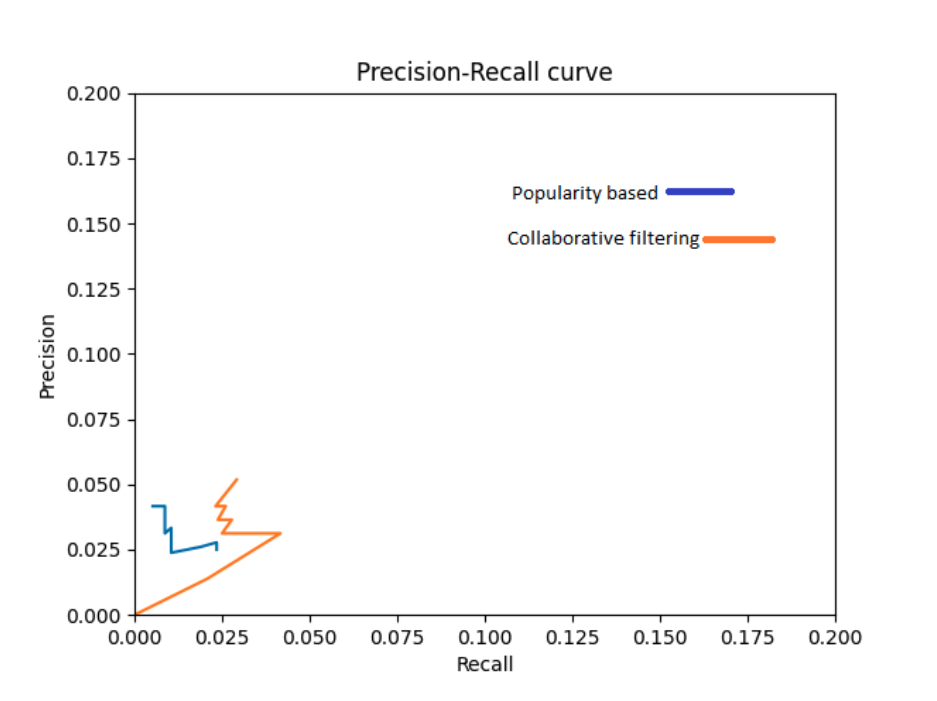
\includegraphics[width=0.8\textwidth]{evaluation}
    \caption{Precision-Recall curve.}
    \label{fig:evaluation}
\end{figure}%

The results have been evaluated using a simple technique. The unique user ID ranges from 0 to 3862. A number of tests have been run to cover the whole range of user ID and results produced successfully. This shows that the system can make recommendations in all situations. Further, a verification is carried out by looking at the list of dataset and counting the number of listens, which showed that the result of popularity-based should be correct.
Similarly, an attempt has been made to trace out how many times the result shown by item-similarity approach appears in the dataset for a simple verification of the results. If it recommends an item which has been rated by only a single user or a few users, then there are chances that it might be producing a wrong result. Such cases were not found, approving of the methods used.


\section{Conclusions, Discussion and further work}

After building this recommender system, there are few things that can be outlined, which are crucial for a collaborative recommendation system. First of all, a dataset containing the ratings provided by the user is a must. This is also called user-interaction data and it is required  for a collaborative approach. This approach is based on similarity of users or items and similarity is actually a function of ratings given by the users. There are a number of ways to calculate similarity and so many ways to make predictions. So, in the real world there has to be knowledge of all these methods and one has to be able to use the particular methods best suited for a certain environment or situation. In this project, however, more than evaluating the efficiency of a particular approach,a focus on producing the results has been made.\\

Precision Recall curve in Figure \ref{fig:evaluation} can be helpful in analyzing the performance of popularity and similarity based approaches. From the graph, it can be concluded that similarity based approach gives more accurate results than naive popularity based approach, as the curve for similarity based method shows it works for much higher values of precision and recall compared with the other method.

The system now shows popularity-based and similarity-based recommendations separately. As a further work,popularity-based methods can be used for new users and similarity-based for old users . Thus combining these approaches, a better system can be made suited for both new as well as old users.

\backmatter

\nocite{*}
\bibliographystyle{alphaurl}
\bibliography{main}

% \newpage
\abouttheauthors

\end{document}
